
\documentclass{beamer}
\usepackage[utf8]{inputenc}
\usepackage[ngerman]{babel}
\usepackage{multicol}
\usepackage[utf8]{inputenc}
\usepackage[T1]{fontenc}
\usepackage[ngerman]{babel}
\usepackage{amsmath}
\usepackage{amsfonts}
\usepackage{amssymb}
%\usepackage{paralist}
\usepackage{color}
\usepackage{xcolor}
\usepackage{lmodern}
\usepackage{graphicx}
\usepackage[mediumspace,mediumqspace,squaren]{SIunits} %SI-Einheiten
\usepackage[version=3]{mhchem} %chemische Formeln
\usepackage{tabularx, calc} %Tabellen
\usepackage{multirow} %Tabelle: mehrere Spalten vereinigen
\usepackage{booktabs} %Verbesserung der Tabellenqualität
\usepackage{caption} %Abbildungs- und Tabellenbeschriftung
\usepackage{array} %Matheumgebung ähnlich tabular
\usepackage{pgf}
\usepackage{dcolumn}
\usepackage{beamerthemeshadow}
\usepackage{comment}
\usepackage{framed}
\usepackage{longtable}
\beamersetuncovermixins{\opaqueness<1>{25}}{\opaqueness<2->{15}}
\begin{document}
\title{Bachelorarbeit}
\subtitle{Disambiguierungsstrategien in Dialogsystemen }  
%\title{Disambiguierungsstrategien in Dialogsystemen }
%\subtitle{Bachelorarbeit}
\author{Lena Enzweiler}
\institute{Universität des Saarlandes}
\date{\today} 

\beamertemplatenavigationsymbolsempty

\setbeamertemplate{footline}[frame number]

\frame{\titlepage} 

\section{Einleitung}
\subsection{Dialogsysteme}
\frame{\frametitle{Dialogsysteme}
\begin{figure}[h]
\caption{Funktionweise der odp-s3 Platform der Semvox GmbH}
	%\centering
        \fbox{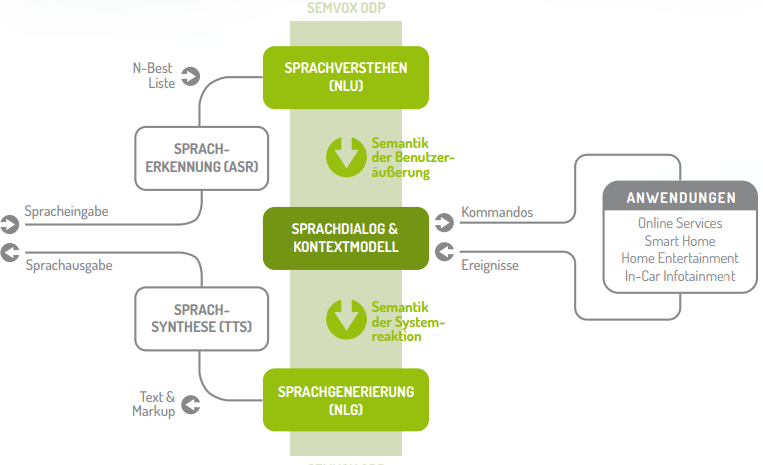
\includegraphics[scale=0.30]{odps3}}
\end{figure}
\begin{itemize}
\item Spracheingabe als semantisches Objekt interpretiert
\item Objekt von Sprachdialog- und Kontextmodell verarbeitet                                                                                                                                                                                                                                                                                                                                                                                                                                                                                                                                                                                                                                                                                                                                                                                                                                                                                                                                                                                                                                                                                                                                                                                                                                                                         
\item Systemreaktion als Sprachausgabe realisiert
\end{itemize} 
}
\subsection{Dialogsysteme im automobilen Bereich}
\frame{\frametitle{Dialogsysteme im automobilen Bereich}
Dialogsysteme im Auto sollten folgende Punkte erfüllen:
\newline
\begin{itemize}
\item Ablenkung während der Fahrt vermeiden
\item alle Informationen verständlich übermitteln
\item einfache und intuitive Bedienung garantieren 
\newline
\end{itemize} 

$\rightarrow$ Sprachäußerungen müssen raffiniert gestaltet werden
}
\subsection{Fokus der Studie}
\frame{\frametitle{Fokus der Studie}
\begin{itemize}
\item ambige Eingaben des Benutzers möglich
\item System muss Mehrdeutigkeit der Eingaben auflösen
\newline
\end{itemize}
$\rightarrow$ Disambiguierung durch geschicktes Nachfragen beim Benutzer
\newline
\newline
%Fokus der Studie:
\begin{block}{Fokus der Studie} Welche Disambiguierungsstrategie eignet sich für Dialogsysteme in einer automobilen Anwendung?  \end{block} 
}
\section{Disambiguierungsstrategien}
\subsection{Disambiguierung}
\frame{\frametitle{Disambiguierung}
Abgrenzung verschiedener Bedeutungen

\begin{figure}[h]
	%\centering
        \fbox{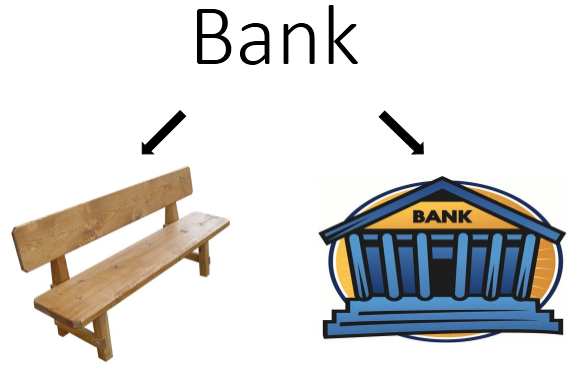
\includegraphics[scale=0.35]{disnomen}}
\end{figure}
}

\subsection{Disambiguierung in Dialogsystemen}
\frame{\frametitle{Disambiguierung in Dialogsystemen}
\begin{figure}[htbp]
	% minipage mit (Blind-)Text
	\begin{minipage}{0.5\textwidth} 
	\begin{itemize}
	\item "Rufe Peter an!"
	\newline
	\item System muss über Peter Meier und Peter Müller disambiguieren
	\newline
	\item unterschiedliche Disambiguierunsstrategien anwendbar
	\newline
	\end{itemize}
	\end{minipage}
	% Auffüllen des Zwischenraums
	\hfill
	% minipage mit Grafik
	\begin{minipage}{0.4\textwidth}
	% \textwidth bezieht sich nun auf die Minipage
	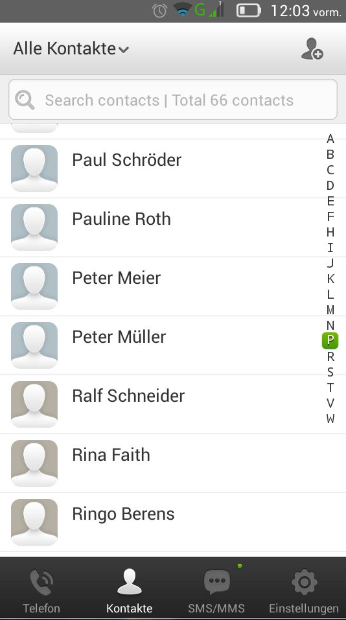
\includegraphics[scale=0.33]{peter}
	\label{Adressbuch} 
	\end{minipage}
% \caption{noch eine Caption}
\end{figure}
$\rightarrow$ 3 Disambiguierungstrategien untersucht
}
\subsection{1. Disambiguierungsstrategie}
\frame{\frametitle{1. Disambiguierungsstrategie: \\Aggregierte Auswahl ohne Pause}

\begin{itemize}
\item alle möglichen Interpretationen in einer Sprachausgabe 
\item keine Pause zwischen Interpretationen
\item auf Auswahl des Benutzers gewartet
\end{itemize}

\begin{table}
\begin{tabular}{l|l }
\textbf{Akteur} &	\textbf{Sprachausgabe}\\
\hline \hline
Benutzer & Rufe Peter an!\\
System & Meinst du Peter Müller oder Peter Meier?\\
Benutzer & Peter Müller.\\
System & Ok, ich werde Peter Müller jetzt anrufen.\\
\end{tabular}
%\caption{Interaktionsbeispiel \texttt{Aggregierte Auswahl ohne Pause}}
\end{table}


}
\subsection{2. Disambiguierungsstrategie}
\frame{\frametitle{2. Disambiguierungsstrategie: \\Aggregierte Auswahl mit Pause}
\begin{itemize}
\item alle möglichen Interpretationen in einer Sprachausgabe 
\item Pause und Nummerierung zwischen Interpretationen
\item auf Auswahl des Benutzers gewartet
\end{itemize}

\begin{table}
\begin{tabular}{l|l }
\textbf{Akteur} &	\textbf{Sprachausgabe}\\
\hline \hline
Benutzer & Rufe Peter an!\\
System & Meinst du [Pause] 1. Peter Müller\\
& [Pause] oder 2. Peter Meier?\\
Benutzer & Erstens \\
System & Ok, ich werde Peter Müller jetzt anrufen.\\
\end{tabular}
%\caption{Interaktionsbeispiel \texttt{Aggregierte Auswahl ohne Pause}}
\end{table} 
}
\subsection{3. Disambiguierungsstrategie}
\frame{\frametitle{3. Disambiguierungsstrategie: \\Sequentielle Auswahl}
\begin{itemize}
\item alle möglichen Interpretationen in einer separaten Sprachausgabe 
\item auf Zustimmung/Ablehnung des Benutzer gewartet
\end{itemize}

\begin{table}
\begin{tabular}{l|l }
\textbf{Akteur} &	\textbf{Sprachausgabe}\\
\hline \hline
Benutzer & Rufe Peter an!\\
System & Meinst du Peter Meier?\\
Benutzer & Nein.\\
System & Meinst du Peter Müller?\\
Benutzer & Ja.\\
System & Ok, ich werde Peter Müller jetzt anrufen.\\
\end{tabular}
%\caption{Interaktionsbeispiel \texttt{Aggregierte Auswahl ohne Pause}}
\end{table} 
}
\section{Versuch 1}
\subsection{Versuchsbeschreibung}
\frame{\frametitle{Kurzbeschreibung}
\begin{itemize}
\item Probanden fahren ein Rennspiel (hohe kognitive Belastung)
\item parellele Interaktion mit Dialogsystem                                                                                                                                                                                                                                                                                                                                                                                                                                                                                                                                                                                                                                                                                                                                                                                                                                                                                                                                                                                                                                                                                                                                                                                                                                                                               
\item alle Disambiguierungsstrategien pro Versuchsperson untersucht
\newline
\item Probanden interagieren ohne Rennspiel (geringe kognitive Belastung) 
\item eine Disambiguierungsstrategie zufällig getestet
\newline
\end{itemize}
$\rightarrow$ Disambiguierungsstrategien auf Effizienz und Beliebtheit untersucht \newline
$\rightarrow$ Ergebnisse mit und ohne Rennspiel werden miteinander verglichen 
}

\frame{\frametitle{Wizard-of-Oz}
\begin{itemize}
\item Die Existenz eines funktionierenden Systems wird vorgetäuscht
\newline
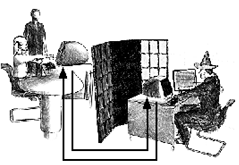
\includegraphics[scale=0.6]{woz}
\newline
\item Versuchspersonen wird der Eindruck verliehen, sie würde mit einem echten Dialogsystem interagieren
\item echtes Dialogsystem durch Versuchsleiter simuliert
\item Control Panel entwickelt, mit welchem Sprachausgaben ausgeben werden können
\end{itemize}
}

\frame{\frametitle{Testszenario}
\begin{itemize}
\item Versuchspersonen sollen erfolgreich per Sprachsteuerung einen Anruf aufbauen
\item insgesamt sollen vier Personen angerufen werden
\item nach Anrufinitialisierung wird simuliert, dass die Spracheingabe zu unspezifisch ist \newline $\rightarrow$ System stellt Rückfrage um zum Beispiel über mehrere mögliche Kontakte oder Telefonnummern zu disambiguieren
\item Nachfrage erfolgt in unterschiedlichen Strategien
\end{itemize}
\begin{block}{Beispiel} Benutzer: "Rufe Anke an" \newline System:\quad "Meinst du Anke Meier oder Schuhmacher?" \end{block} 

}

\frame{\frametitle{Testszenario}
\begin{figure}[htbp]
	% minipage mit (Blind-)Text
	\begin{minipage}{0.5\textwidth} 
		\begin{itemize}
			\item relevante Personenangaben (Slots) werden über ein Personenprofil angezeigt.
			\item pro Anruf werden jeweils 2 Slots abgefragt.
			\item die zufüllenden Slots unterscheiden sich pro anzurufenden Kontakt
			\item Rückfragen sind so generiert, dass der Slot an zweiter Stelle der zu füllende ist 
		\end{itemize}
	\end{minipage}
	\hfill
	\begin{minipage}{0.4\textwidth}
	\fbox{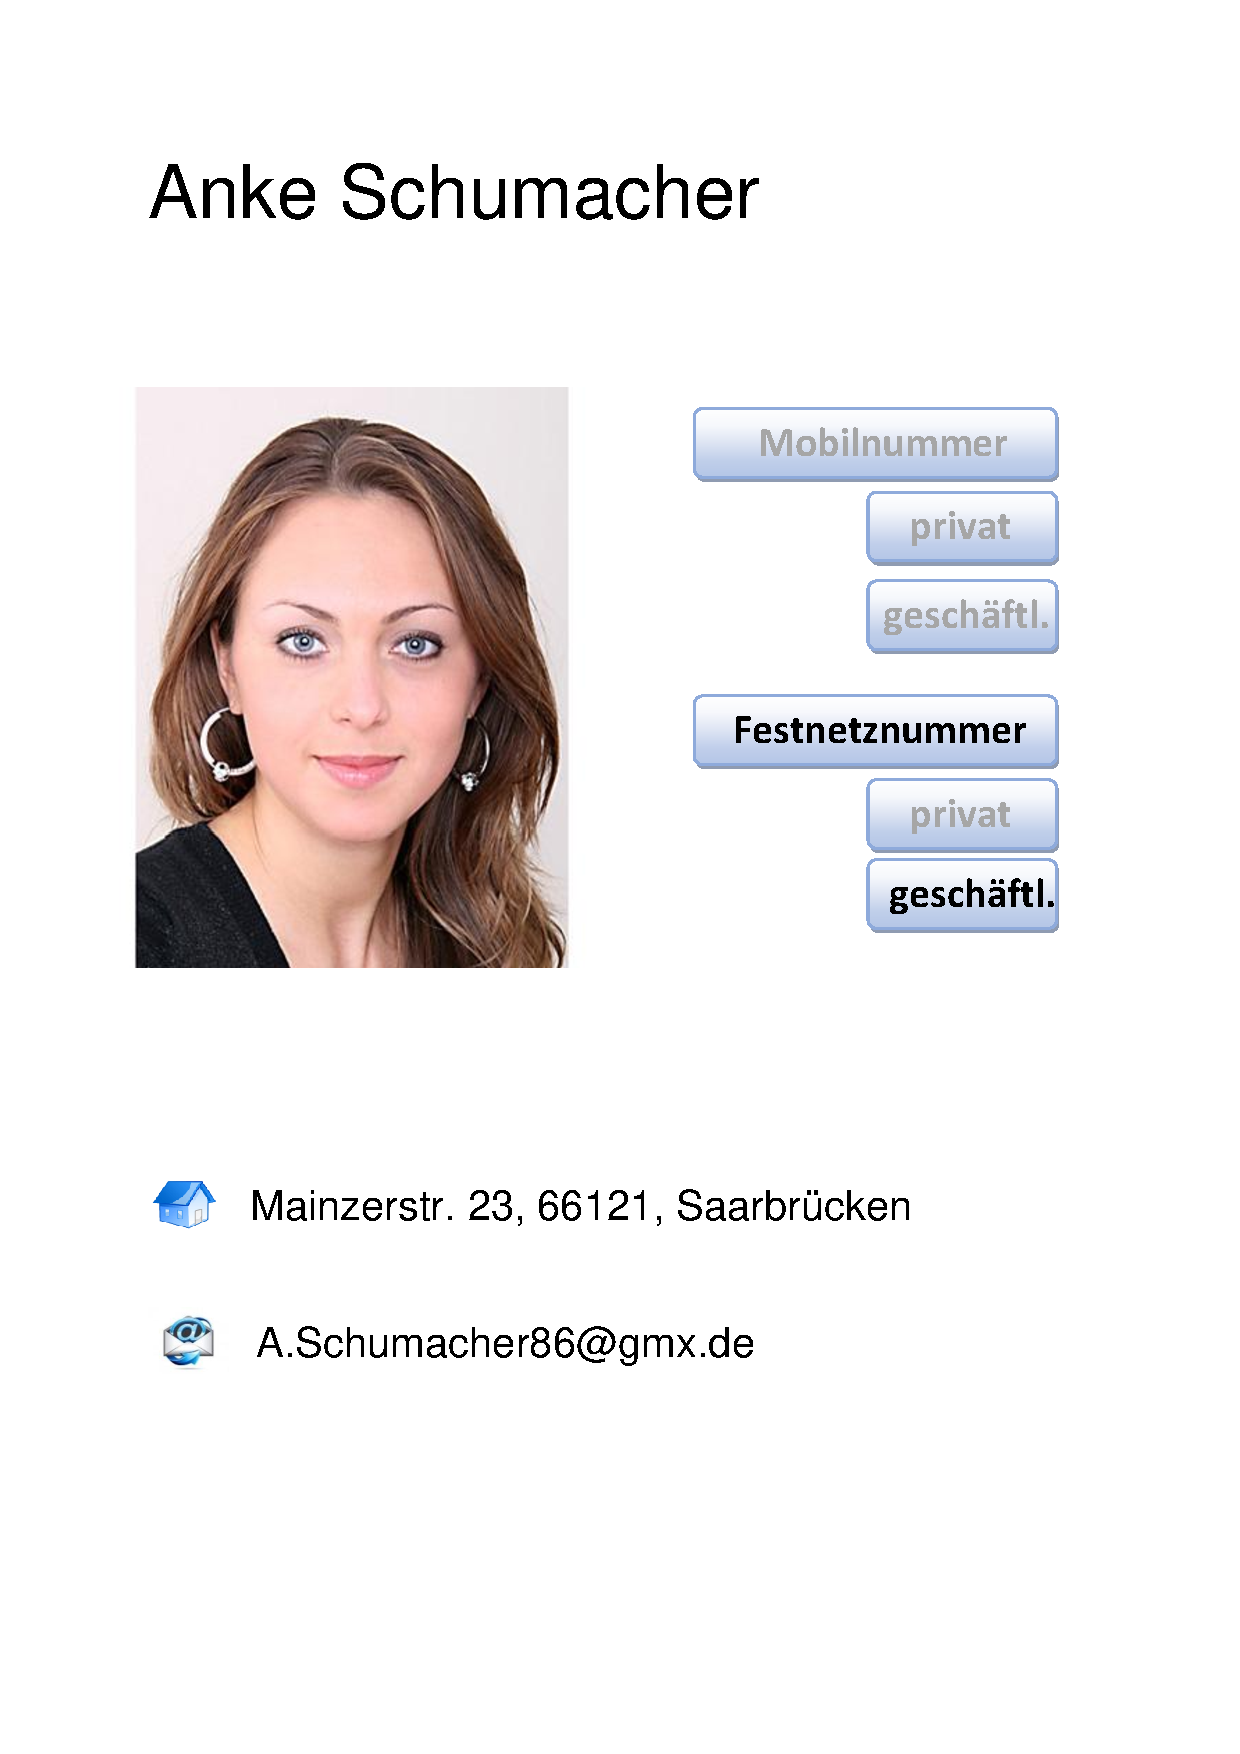
\includegraphics[scale=0.21]{Anke}}
	\label{Adressbuch} 
	\end{minipage}
% \caption{noch eine Caption}
\end{figure}
}

\frame{\frametitle{Versuchsaufbau}
\begin{itemize}
\item Versuchspersonen fahren ein Rennspiel. \newline $\rightarrow$ Fahrsimulation
\item Rennspiel: Need for Speed: Shift
\item Rennspiel wird mit Lenkrad inklusive Gas- und Bremspedal gespielt \newline $\rightarrow$ realitätsgetreues Gefühl
\item Es wird im Einzelrennen mit jeweils 5 Gegnern gespielt
\item Versuchspersonen sollen möglichst hohe Platzierung erreichen \newline $\rightarrow$ Anstrengung und Konzentration soll hohe kognitive Belastung verursachen
\end{itemize} 
}

\frame{\frametitle{Versuchsaufbau - Rennspiel}
\begin{figure}[h]
\caption{Need for Speed - Shift}
	%\centering
        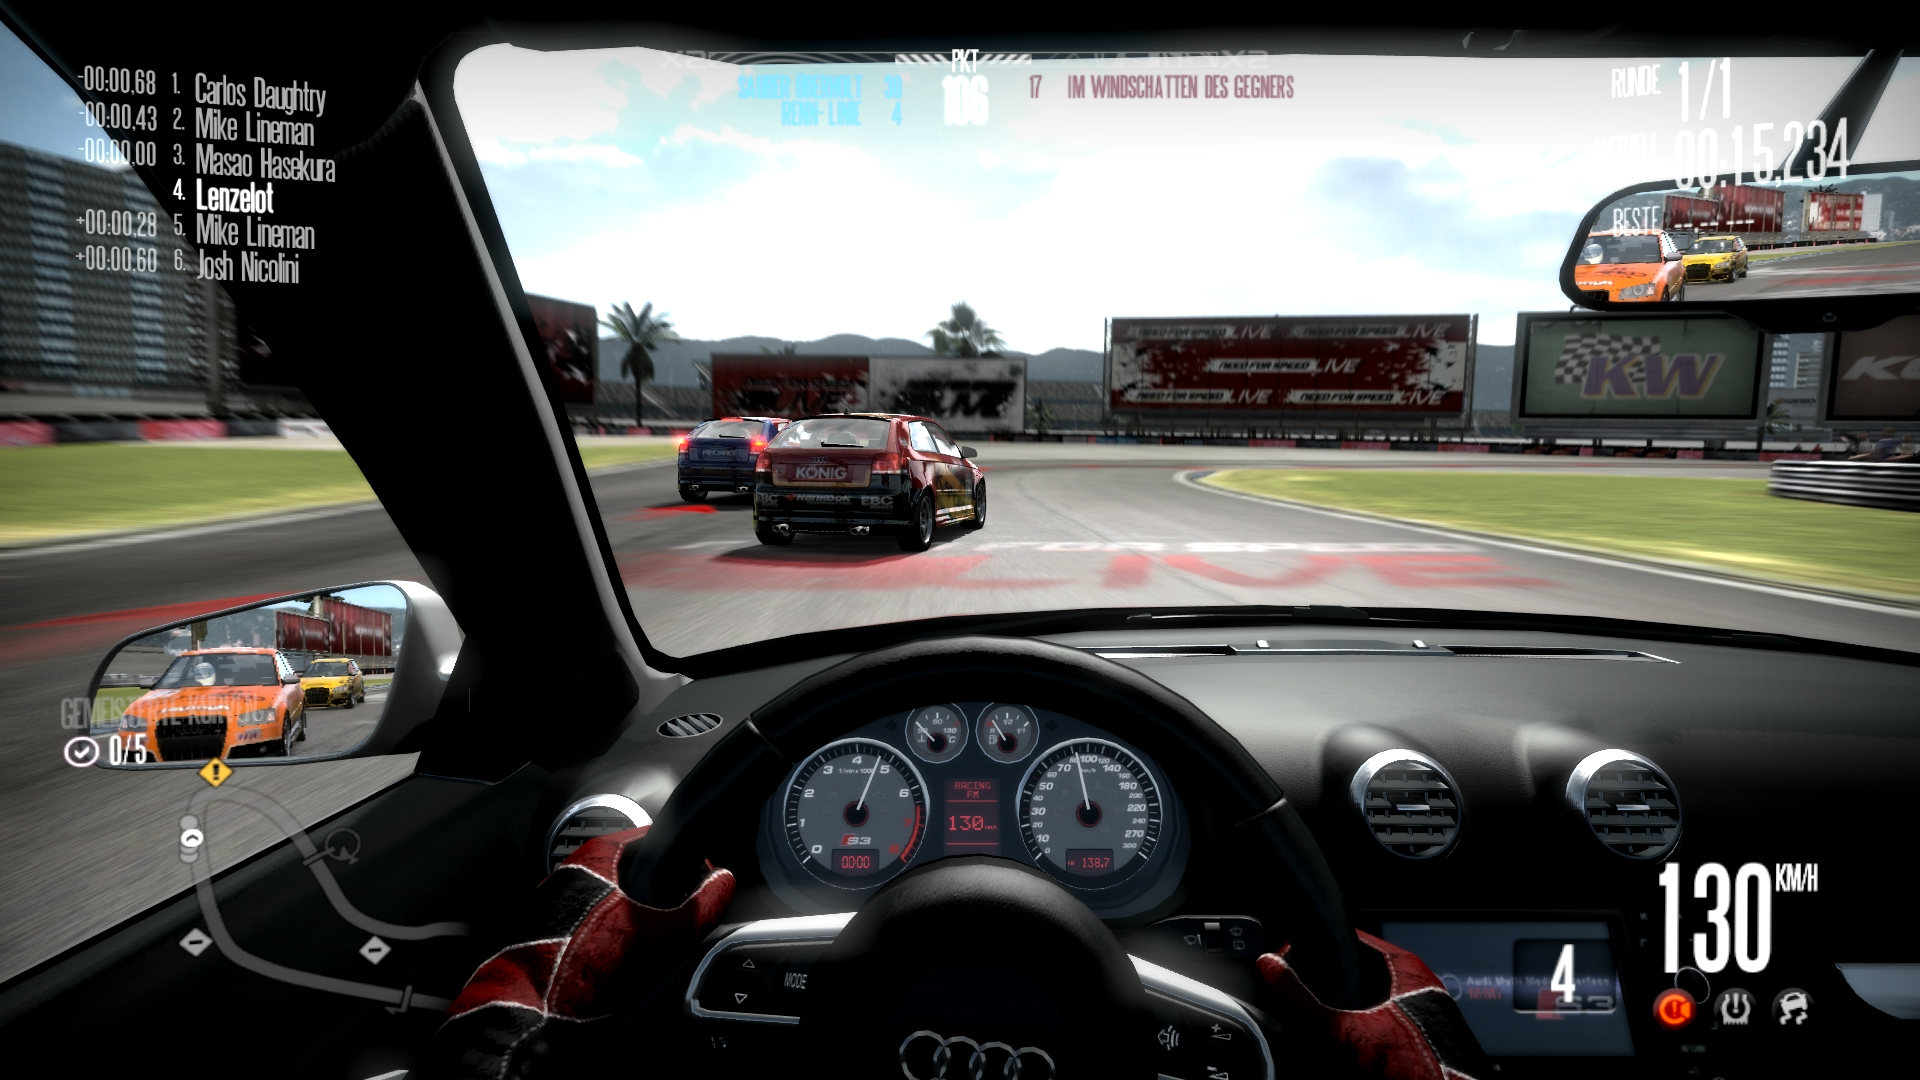
\includegraphics[scale=0.2]{nfs}
\end{figure}
}

\frame{\frametitle{Versuchsaufbau - Überblick}
\begin{table}
\begin{tabular}{l|l|l|l|l}
\textbf{Vorrunde}&\textbf{1. Runde}&\textbf{2. Runde} &\textbf{3. Runde} &\textbf{4. Runde}\\
\hline \hline
Rennspiel & Rennspiel & Rennspiel & Rennspiel &\\
 & Anruf Anke & Anruf Peter & Anruf Fritz & Anruf Kim \\
\end{tabular}
%\caption{Interaktionsbeispiel \texttt{Aggregierte Auswahl ohne Pause}}
\end{table}
\begin{itemize}
\item Vorrunde zum Einspielen
\item Runde 1-3: Rennspiel mit paralleler Systeminteraktion \newline $\rightarrow $ hohe kognitive Belastung
\item Runde 4: nur Systeminteraktion \newline $\rightarrow $ geringe kognitive Belastung
\end{itemize}
}

\frame{\frametitle{Versuchsdesign}
\begin{table}
\begin{tabular}{l|l|l|l}
\textbf{Aufteilung}&\textbf{Strecke 1}&\textbf{Strecke 2} &\textbf{Strecke 3}\\
\hline \hline
1. Gruppe & Strategie A & Strategie B & Strategie C \\
2. Gruppe & Strategie B & Strategie C & Strategie A\\
3. Gruppe  & Strategie C & Strategie A & Strategie B\\
4. Gruppe   & keine Strecke & keine Strecke & keine Strecke\\ 
\end{tabular}
%\caption{Interaktionsbeispiel \texttt{Aggregierte Auswahl ohne Pause}}
\end{table}
\begin{itemize}
\item 3 verschiedene Strecken, um Lerneffekt auszuschließen
\item jede Strecke mit unterschiedlicher Disambiguierungsstrategie
\item um Zeiten besser zu vergleichen: \newline $\rightarrow$ Disambiguierungsstrategien werden auf Strecken verteilt  \newline $\rightarrow$ Versuchspersonen werden in Gruppen (1-3) aufgeteilt
\item Die Strecken werden in gleicher Reihenfolge gefahren
\item Gruppe 4 führt das Testszenario mit zufälliger Strategie aus. 
\end{itemize}
}

\subsection{Control Panel}
\frame{\frametitle{Control Panel}
\begin{itemize}
\item entwickelt um ein laufendes Dialogsystem zu simulieren
\item verschiedene Sprachausgaben können per Mausklick abgespielt werden
\begin{figure}
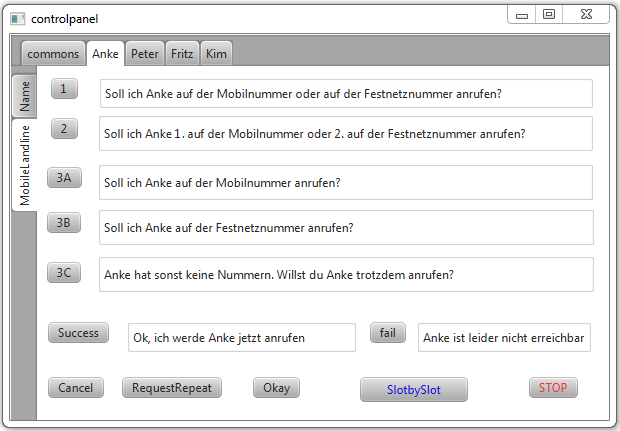
\includegraphics[scale=0.4]{controlpanel}
\end{figure}
\end{itemize}
}
\subsection{Versuchspersonen}
\frame{\frametitle{Versuchspersonen}
\begin{enumerate}
\item hello
\item world
\end{enumerate}
}
\subsection{Auswertung}
\frame{\frametitle{Vorahnung}
\textsl{"The wise man avoids evil by anticipating it" (Publilius Syrus)}
\newline

Vorahnung ist lebenswichtig
\begin{itemize}
\item kein Halten von gef\"ahrlichen Tieren als Haustiere
\item keine Spazierg\"ange bei Gewitter                                                                                                                                                                                                                                                                                                                                                                                                                                                                                                                                                                                                                                                                                                                                                                                                                                                                                                                                                                                                                                                                                                                                                                                                                                                                               
\item Reflexe aus\"uben
\end{itemize} 
}
\subsection{Resultat}
\frame{\frametitle{Vorahnung}
\textsl{"The wise man avoids evil by anticipating it" (Publilius Syrus)}
\newline

Vorahnung ist lebenswichtig
\begin{itemize}
\item kein Halten von gef\"ahrlichen Tieren als Haustiere
\item keine Spazierg\"ange bei Gewitter                                                                                                                                                                                                                                                                                                                                                                                                                                                                                                                                                                                                                                                                                                                                                                                                                                                                                                                                                                                                                                                                                                                                                                                                                                                                               
\item Reflexe aus\"uben
\end{itemize} 
}
\section{Versuch 2}
\subsection{Versuchsbeschreibung}
\frame{\frametitle{Vorahnung}
\textsl{"The wise man avoids evil by anticipating it" (Publilius Syrus)}
\newline

Vorahnung ist lebenswichtig
\begin{itemize}
\item kein Halten von gef\"ahrlichen Tieren als Haustiere
\item keine Spazierg\"ange bei Gewitter                                                                                                                                                                                                                                                                                                                                                                                                                                                                                                                                                                                                                                                                                                                                                                                                                                                                                                                                                                                                                                                                                                                                                                                                                                                                               
\item Reflexe aus\"uben
\end{itemize} 
}
\begin{comment}
\subsection{Versuchsaufbau}
\frame{\frametitle{Vorahnung}
\textsl{"The wise man avoids evil by anticipating it" (Publilius Syrus)}
\newline

Vorahnung ist lebenswichtig
\begin{itemize}
\item kein Halten von gef\"ahrlichen Tieren als Haustiere
\item keine Spazierg\"ange bei Gewitter                                                                                                                                                                                                                                                                                                                                                                                                                                                                                                                                                                                                                                                                                                                                                                                                                                                                                                                                                                                                                                                                                                                                                                                                                                                                               
\item Reflexe aus\"uben
\end{itemize} 
}
\subsection{Versuchsdesign}
\frame{\frametitle{Vorahnung}
\textsl{"The wise man avoids evil by anticipating it" (Publilius Syrus)}
\newline

Vorahnung ist lebenswichtig
\begin{itemize}
\item kein Halten von gef\"ahrlichen Tieren als Haustiere
\item keine Spazierg\"ange bei Gewitter                                                                                                                                                                                                                                                                                                                                                                                                                                                                                                                                                                                                                                                                                                                                                                                                                                                                                                                                                                                                                                                                                                                                                                                                                                                                               
\item Reflexe aus\"uben
\end{itemize} 
}
\end{comment}
\subsection{Control Panel}
\frame{\frametitle{Vorahnung}
\textsl{"The wise man avoids evil by anticipating it" (Publilius Syrus)}
\newline

Vorahnung ist lebenswichtig
\begin{itemize}
\item kein Halten von gef\"ahrlichen Tieren als Haustiere
\item keine Spazierg\"ange bei Gewitter                                                                                                                                                                                                                                                                                                                                                                                                                                                                                                                                                                                                                                                                                                                                                                                                                                                                                                                                                                                                                                                                                                                                                                                                                                                                               
\item Reflexe aus\"uben
\end{itemize} 
}
\subsection{Versuchspersonen}
\frame{\frametitle{Vorahnung}
\textsl{"The wise man avoids evil by anticipating it" (Publilius Syrus)}
\newline

Vorahnung ist lebenswichtig
\begin{itemize}
\item kein Halten von gef\"ahrlichen Tieren als Haustiere
\item keine Spazierg\"ange bei Gewitter                                                                                                                                                                                                                                                                                                                                                                                                                                                                                                                                                                                                                                                                                                                                                                                                                                                                                                                                                                                                                                                                                                                                                                                                                                                                               
\item Reflexe aus\"uben
\end{itemize} 
}

\subsection{Auswertung}
\frame{\frametitle{Vorahnung}
\textsl{"The wise man avoids evil by anticipating it" (Publilius Syrus)}
\newline

Vorahnung ist lebenswichtig
\begin{itemize}
\item kein Halten von gef\"ahrlichen Tieren als Haustiere
\item keine Spazierg\"ange bei Gewitter                                                                                                                                                                                                                                                                                                                                                                                                                                                                                                                                                                                                                                                                                                                                                                                                                                                                                                                                                                                                                                                                                                                                                                                                                                                                               
\item Reflexe aus\"uben
\end{itemize} 
}
\subsection{Resultat}
\frame{\frametitle{Vorahnung}
\textsl{"The wise man avoids evil by anticipating it" (Publilius Syrus)}
\newline

Vorahnung ist lebenswichtig
\begin{itemize}
\item kein Halten von gef\"ahrlichen Tieren als Haustiere
\item keine Spazierg\"ange bei Gewitter                                                                                                                                                                                                                                                                                                                                                                                                                                                                                                                                                                                                                                                                                                                                                                                                                                                                                                                                                                                                                                                                                                                                                                                                                                                                               
\item Reflexe aus\"uben
\end{itemize} 
}

\section{Ergebnisse}
\frame{\frametitle{Vorahnung}
\textsl{"The wise man avoids evil by anticipating it" (Publilius Syrus)}
\newline

Vorahnung ist lebenswichtig
\begin{itemize}
\item kein Halten von gef\"ahrlichen Tieren als Haustiere
\item keine Spazierg\"ange bei Gewitter                                                                                                                                                                                                                                                                                                                                                                                                                                                                                                                                                                                                                                                                                                                                                                                                                                                                                                                                                                                                                                                                                                                                                                                                                                                                               
\item Reflexe aus\"uben
\end{itemize} 
}
\section{Fazit}
\frame{\frametitle{Vorahnung}
\textsl{"The wise man avoids evil by anticipating it" (Publilius Syrus)}
\newline

Vorahnung ist lebenswichtig
\begin{itemize}
\item kein Halten von gef\"ahrlichen Tieren als Haustiere
\item keine Spazierg\"ange bei Gewitter                                                                                                                                                                                                                                                                                                                                                                                                                                                                                                                                                                                                                                                                                                                                                                                                                                                                                                                                                                                                                                                                                                                                                                                                                                                                               
\item Reflexe aus\"uben
\end{itemize} 
}

\end{document}

